\documentclass{beamer}

\usepackage[utf8]{inputenc}
\usepackage[T1]{fontenc}
\usepackage{amsmath}
\usepackage{amsthm}
\usepackage{dsfont}
\usepackage{graphicx}
\usepackage{interval}
\usepackage{color}
\usepackage{xcolor,colortbl}
\usepackage[style=authoryear, maxcitenames=11, mincitenames=11, natbib=true, uniquename=false, uniquelist=false]{biblatex}
\addbibresource{main.bib}
\usepackage{multirow}
\usepackage{booktabs}
\usepackage{tikz}
\usetikzlibrary{patterns}
\usetikzlibrary{positioning}
\usetikzlibrary{decorations.pathreplacing,angles,quotes}
\usepgflibrary{arrows.meta,shapes.geometric}
\usepackage{algorithm}
\usepackage{algorithmicx}
\usepackage[noend]{algpseudocode}
\usepackage{dirtytalk}
\usepackage{hyperref}

\beamertemplatenavigationsymbolsempty%
\addtobeamertemplate{navigation symbols}{}{%
    \usebeamerfont{footline}%
    \usebeamercolor[fg]{footline}%
    \hspace{1em}%
    \insertframenumber/\inserttotalframenumber%
}

\author{Florian Fontan}
\title{Advanced Models and Methods in Operations Research \\ Dynamic programming}
\date{November 7, 2023}

\begin{document}

\newcommand{\customcite}[1]{\citetitle{#1}, \citeauthor{#1}, \citeyear{#1}}

\AtBeginSection[]
{%
  \begin{frame}<beamer>
    \frametitle{Table of contents}
    \tableofcontents[currentsection]
  \end{frame}
}

\maketitle

\section{Introduction}

\begin{frame}
  \frametitle{Me}

  \begin{itemize}
    \item Former student of ORCO (2015--2016)
    \item PhD in Operations Research
    \item Engineer at Artelys: \url{https://www.artelys.com/}
      \begin{itemize}
        \item Artelys is an independent company specialized in optimization, decision support and modeling
        \item Design and implementation of optimization algorithms for industrial clients
        \item Development for the NLP/MINLP solver Artelys Knitro \url{https://www.artelys.com/solvers/knitro/}
      \end{itemize}
    \item My GitHub: \url{https://github.com/fontanf/}
  \end{itemize}
\end{frame}

\begin{frame}
  \frametitle{Organization}
  \begin{itemize}
    \item 4 classes with me:
      \begin{itemize}
        \item Dynamic programming
        \item Heuristic tree search
        \item Column generation heuristics
        \item Project presentations
      \end{itemize}
    \item 1.5 hours lecture / 1.5 hours practical training
      \item Goal of the classes: understanding the theory of the methods and being able to implement them to solve practical problems
  \end{itemize}
\end{frame}

\begin{frame}
  \frametitle{Organization}
  \begin{itemize}
    \item Evaluation:
      \begin{itemize}
        \item Not in the final exam
        \item Project by groups of 3 or 4
        \item Implementation of the algorithms studied in the classes
        \item First deadline with feedbacks
        \item Second deadline with final grade
        \item Please do not put your code on a public repository
        \item You can keep it on a private repository. It can be valuable if you decide to apply for a company some day
      \end{itemize}
    \item All materials (slides, projects\dots) are online \url{https://github.com/fontanf/teaching}
    \item E-mail: \href{mailto:dev@florian-fontan.fr}{dev@florian-fontan.fr}
  \end{itemize}
\end{frame}

\section{The partition problem and the subset sum problem}

\begin{frame}
  \frametitle{Problem definition}

  \begin{block}{Partition problem}
    \begin{itemize}
      \item Instance: $n$ items with weight \alert{$w_j$}, $j = 1, \dots, n$.
      \item Question: is it possible to partition the set of items into two subsets of equal weights?
    \end{itemize}
  \end{block}

  \pause

  We consider a slightly more general variant:
  \begin{block}{Subset sum problem (decision version)}
    \begin{itemize}
      \item Instance:
        \begin{itemize}
          \item $n$ items with weight \alert{$w_j$}, $j = 1, \dots, n$
          \item a capacity \alert{$C$}
        \end{itemize}
      \item Question: is there a subset of items with total weight $C$?
    \end{itemize}
  \end{block}

  \pause
  Link between the partition problem and the subset sum problem?
  \pause
  The partition problem is a subset sum problem with capacity $C = \frac{1}{2} \sum_{j = 1}^n w_j$.
\end{frame}

\begin{frame}
  \frametitle{Recursive function}

  For all $j = 0, \dots, n$, $c = 0, \dots, C$, let us define:
  \begin{displaymath}
    F(j, c) =
    \left\{
      \begin{array}{ll}
        \text{True} & \text{if among items $1, \dots, j$, there exists} \\
        & \text{a subset of items with total weight $c$} \\
        \text{False} & \text{otherwise}
      \end{array}
    \right.
  \end{displaymath}

  \pause
  What is the value of
  \begin{itemize}
    \item $F(0, 0)$? \pause True \pause
    \item $F(0, c)$? \pause True for $c = 0$, False otherwise \pause
    \item $F(j, 0)$? \pause True \pause
  \end{itemize}

  What is the relation between the subset sum problem and $F$? \pause

  The subset sum problem is equivalent to determining the value of $F(n, C)$.
\end{frame}

\begin{frame}
  \frametitle{Computing $F(n, C)$}

  We compute $F(j, c)$ with the following recursive formula:
  \begin{displaymath}
    F(j, c) =
    \left\{
      \begin{array}{ll}
        \text{True} & \text{if $j = 0$ and $c = 0$} \\
        \text{False} & \text{if $j = 0$ and $c \neq 0$} \\
        F(j - 1, c) & if \text{$j \neq 0$ and $c < w_j$} \\
        F(j - 1, c) & \text{otherwise} \\
        \text{or } F(j - 1, c - w_j) &
      \end{array}
    \right.
  \end{displaymath}
\end{frame}

\begin{frame}
  \frametitle{Divide-and-conquer}

  \small
  We can now solve the subset sum problem with a divide-and-conquer algorithm:

  \begin{minipage}[t]{0.68\linewidth}
    \begin{algorithmic}
      \Function{F}{$w$, $j$, $c$}
      \If {$j == 0$}
      \If {$c == 0$}
      \State\Return$True$
      \Else{}
      \State\Return$False$
      \EndIf
      \ElsIf {$c < w_j$}
      \State\Return$F(j - 1, c)$
      \Else{}
      \State\Return$F(j - 1, c) \text{ or } F(j - 1, c - w[j])$
      \EndIf
      \EndFunction{}
      \Function{subsetsum}{$w$, $C$}
      \State\Return{} $F(w, n, C)$
      \EndFunction{}
    \end{algorithmic}
  \end{minipage}
  \hfill
  \begin{minipage}[t]{0.28\linewidth}
    \begin{itemize}
      \item \pause Time complexity? \pause $O(2^n)$
      \item \pause Space complexity? \pause $O(n)$
    \end{itemize}
  \end{minipage}

  \bigskip

  \pause Is there a way to improve the time complexity?
\end{frame}

\begin{frame}
  \frametitle{Divide-and-conquer example}
  Consider an instance $I$ of the subset sum problem with 
  \begin{itemize}
    \item $n = 103$
    \item $C = 1000$
    \item $w_{101} = 30$, $w_{102} = 20$, $w_{103} = 10$.
  \end{itemize}

  \begin{center}
    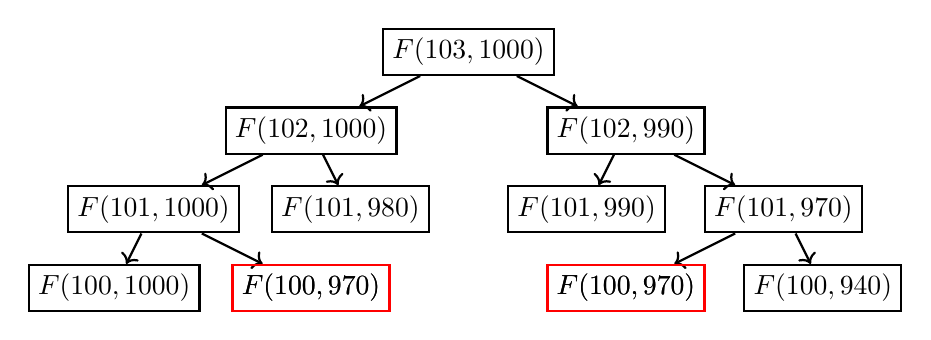
\begin{tikzpicture}
      \onslide<1->{%
        \node[draw=black, thick, rectangle] (103-1000) at (0,0) {$F(103, 1000)$};
      }

      \onslide<2->{%
        \node[draw=black, thick, rectangle] (102-1000) at (-2,-1) {$F(102, 1000)$};
        \node[draw=black, thick, rectangle] (102-990) at (2,-1) {$F(102, 990$)};
        \draw [thick, draw=black, ->] (103-1000) -- (102-1000);
        \draw [thick, draw=black, ->] (103-1000) -- (102-990);
      }

      \onslide<3->{%
        \node[draw=black, thick, rectangle] (101-1000) at (-4,-2) {$F(101, 1000)$};
        \node[draw=black, thick, rectangle] (101-980) at (-1.5,-2) {$F(101, 980$)};
        \draw [thick, draw=black, ->] (102-1000) -- (101-1000);
        \draw [thick, draw=black, ->] (102-1000) -- (101-980);

        \node[draw=black, thick, rectangle] (101-990) at (1.5,-2) {$F(101, 990)$};
        \node[draw=black, thick, rectangle] (101-970) at (4,-2) {$F(101, 970$)};
        \draw [thick, draw=black, ->] (102-990) -- (101-990);
        \draw [thick, draw=black, ->] (102-990) -- (101-970);
      }

      \onslide<4->{%
        \node[draw=black, thick, rectangle] (100-1000) at (-4.5,-3) {$F(100, 1000)$};
        \node[draw=black, thick, rectangle] (100-970) at (-2,-3) {$F(100, 970$)};
        \draw [thick, draw=black, ->] (101-1000) -- (100-1000);
        \draw [thick, draw=black, ->] (101-1000) -- (100-970);

        \node[draw=black, thick, rectangle] (100-970-2) at (2,-3) {$F(100, 970)$};
        \node[draw=black, thick, rectangle] (100-940) at (4.5,-3) {$F(100, 940$)};
        \draw [thick, draw=black, ->] (101-970) -- (100-970-2);
        \draw [thick, draw=black, ->] (101-970) -- (100-940);
      }

      \onslide<5->{%
        \node[draw=red, thick, rectangle] (100-970) at (-2,-3) {$F(100, 970$)};
        \node[draw=red, thick, rectangle] (100-970-2) at (2,-3) {$F(100, 970)$};
      }
    \end{tikzpicture}
  \end{center}

  \onslide<6->{%
    The same subproblems might be solved multiple times!
  }
\end{frame}

\begin{frame}
  \frametitle{Dynamic programming: recursive implementation (top-down)}

  \footnotesize
  Same algorithm as before, but now we store the results of the subproblems to avoid solving multiple times the same subproblems:
  \begin{minipage}[t]{0.75\linewidth}
    \footnotesize
    \begin{algorithmic}
      \Procedure{F}{w, T, j, c}
      \If {$T[j][c] == \mathrm{NULL}$}
      \If {$j == 0$}
      \If {$c == 0$}
      \State$T[j][c] \gets \text{True}$
      \Else{}
      \State$T[j][c] \gets \text{False}$
      \EndIf
      \ElsIf {$c < w[j]$}
      \State$T[j][c] \gets F(j - 1, c)$
      \Else{}
      \State$T[j][c] \gets F(j - 1, c) \text{ or } F(j - 1, c - w[j])$
      \EndIf
      \EndIf
      \State\Return$T[j][c]$
      \EndProcedure{}
      \Procedure{subsetsum}{w, C}
      \State$T \gets$ array of size $(n + 1) \times (C + 1)$ initialized at NULL
      \State\Return$F(w, T, n, C)$
      \EndProcedure{}
    \end{algorithmic}
  \end{minipage}
  \hfill
  \begin{minipage}[t]{0.24\linewidth}
    \footnotesize
    \begin{itemize}
      \item \pause Time complexity? \pause $O(nC)$
      \item \pause Space complexity? \pause $O(nC)$
    \end{itemize}
  \end{minipage}
\end{frame}

\begin{frame}
  \frametitle{Dynamic programming}

  \begin{block}{Dynamic programming}
    Solving a problem recursively and storing the results of the subproblems to avoid recomputing them multiple times.
  \end{block}
\end{frame}

\begin{frame}
  \frametitle{Dynamic programming: iterative implementation (bottom-up)}

  \begin{algorithmic}
    \Procedure{subsetsum}{w, C}
    \State$T \gets$ array of size $(n + 1) \times (C + 1)$ initialized at NULL
    \State$T[0][0] \gets \text{True}$
    \For {$c = 1, \dots, C$}
    \State$T[0][c] \gets \text{False}$
    \EndFor
    \For {$j = 1, \dots, n$}
    \For {$c = 0, \dots, w[j] - 1$}
    \State$T[j][c] \gets T[j - 1][c]$
    \EndFor
    \For {$c = w[j], \dots, C$}
    \State$T[j][c] \gets T[j - 1][c] \text{ or } T[j - 1][c - w[j]]$
    \EndFor
    \EndFor
    \State\Return{}$T[n, C]$
    \EndProcedure{}
  \end{algorithmic}

  \begin{itemize}
    \item \pause Time complexity? \pause $O(nC)$
    \item \pause Space complexity? \pause $O(nC)$
    \item \pause In practice, $10$ times faster than the recursive implementation
  \end{itemize}

\end{frame}

\begin{frame}
  \frametitle{Dynamic programming example}

  Instance:
  \begin{itemize}
    \item $n = 5$, $w = \{ 4, 11, 6, 8, 7 \}$
    \item $C = 17$
  \end{itemize}

  \pause

  Reminder:
  \begin{displaymath}
    F(j, c) =
    \left\{
      \begin{array}{ll}
        \text{True} & \text{if $j = 0$ and $c = 0$} \\
        \text{False} & \text{if $j = 0$ and $c \neq 0$} \\
        F(j - 1, c) & if \text{$j \neq 0$ and $c < w_j$} \\
        F(j - 1, c) & \text{otherwise} \\
        \text{or } F(j - 1, c - w_j) &
      \end{array}
    \right.
  \end{displaymath}

  \small
  \begin{center}
    \begin{tabular}{cp{0.001cm}p{0.001cm}p{0.001cm}p{0.001cm}p{0.001cm}p{0.001cm}p{0.001cm}p{0.001cm}p{0.001cm}p{0.001cm}p{0.001cm}p{0.001cm}p{0.001cm}p{0.001cm}p{0.001cm}p{0.001cm}p{0.001cm}p{0.001cm}}
      \toprule
      j / c & 0 & 1 & 2 & 3 & 4 & 5 & 6 & 7 & 8 & 9 & 10 & 11 & 12 & 13 & 14 & 15 & 16 & 17 \\
      \midrule
      \onslide<3->{0     & T & F & F & F & F & F & F & F & F & F & F  & F  & F  & F  & F  & F  & F  & F } \\
      \onslide<4->{1     & T & F & F & F & T & F & F & F & F & F & F  & F  & F  & F  & F  & F  & F  & F }  \\
      \onslide<5->{2     & T & F & F & F & T & F & F & F & F & F & F  & T  & F  & F  & F  & T  & F  & F }  \\
      \onslide<6->{3     & T & F & F & F & T & F & T & F & F & F & T  & T  & F  & F  & F  & T  & F  & T }  \\
      \onslide<7->{4     & T & F & F & F & T & F & T & F & T & F & T  & T  & T  & F  & T  & T  & F  & T }  \\
      \onslide<8->{5     & T & F & F & F & T & F & T & T & T & F & T  & T  & T  & T  & T  & T  & F  & T }  \\
      \bottomrule
    \end{tabular}
  \end{center}
\end{frame}

\begin{frame}
  \frametitle{Retrieving the solution with backtracking}

  The algorithms presented in the previous slides only return True or False. In case the answer is True, we would also like to get a solution, \textit{i.e.}\ a subset of items with total weight $C$.

  $w = \{ 4, 11, 6, 8, 7 \}$

  \small
  \begin{center}
    \begin{tabular}{cp{0.001cm}p{0.001cm}p{0.001cm}p{0.001cm}p{0.001cm}p{0.001cm}p{0.001cm}p{0.001cm}p{0.001cm}p{0.001cm}p{0.001cm}p{0.001cm}p{0.001cm}p{0.001cm}p{0.001cm}p{0.001cm}p{0.001cm}p{0.001cm}}
      \toprule
      j / c & 0 & 1 & 2 & 3 & 4 & 5 & 6 & 7 & 8 & 9 & 10 & 11 & 12 & 13 & 14 & 15 & 16 & 17 \\
      \midrule
      0     & \temporal<11>{T}{\cellcolor{blue!25} T}{\cellcolor{red!25} T} & F & F & F & \temporal<11>{F}{\cellcolor{blue!25} F}{F} & F & F & F & F & F & F  & F  & F  & F  & F  & F  & F  & F  \\
      1     & T & F & F & F & \temporal<9>{T}{\cellcolor{blue!25} T}{\cellcolor{red!25} T} & F & F & F & F & F & F  & F  & F  & F  & F  & F  & F  & F  \\
      2     & T & F & F & F & \temporal<7>{T}{\cellcolor{blue!25} T}{\cellcolor{red!25} T} & F & F & F & F & F & \temporal<7>{F}{\cellcolor{blue!25}F}{F}  & T  & F  & F  & F  & T  & F  & F  \\
      3     & T & F & \temporal<5>{F}{\cellcolor{blue!25} F}{F} & F & T & F & T & F & F & F & \temporal<5>{T}{\cellcolor{blue!25} T}{\cellcolor{red!25} T} & T  & F  & F  & F  & T  & F  & T  \\
      4     & T & F & F & F & T & F & T & F & T & F & \temporal<3>{T}{\cellcolor{blue!25} T}{\cellcolor{red!25} T}  & T  & T  & F  & T  & T  & F  & \temporal<3>{T}{\cellcolor{blue!25} T}{T}  \\
      5     & T & F & F & F & T & F & T & T & T & F & T  & T  & T  & T  & T  & T  & F  & \alt<1>{T}{\cellcolor{red!25} T}  \\
      \bottomrule
    \end{tabular}
  \end{center}

  \onslide<13>{$S = \{5, 3, 1 \}$}
  \pause
\end{frame}

\begin{frame}
  \frametitle{Retrieving the solution with backtracking}

  \begin{algorithmic}
    \Function{SSPbacktracking}{w, C, T}
    \State$S \gets \{ \}$
    \State$c \gets C$
    \State$i \gets n$
    \While{$i > 0$}
    \If {not $T[i-1][c]$}
    \State$S \gets S \cup \{ i \}$
    \State$c \gets c - w[j]$
    \EndIf
    \State {} $i \gets i - 1$
    \EndWhile{}
    \State {} \Return{} S
    \EndFunction{}
  \end{algorithmic}
\end{frame}

\begin{frame}
  \frametitle{Going further}

  \begin{itemize}
    \item Write an algorithm computing $F(n, C)$ which only keeps two lines of the array in memory (spatial complexity $O(C)$)
    \item Write an algorithm computing $F(n, C)$ which only keeps a single line of the array in memory.
    \item How to return a solution when keeping only a single line in memory?
      \begin{itemize}
        \item if the array is stored as an array of integers
        \item if the array is stored as an array of bits
      \end{itemize}
  \end{itemize}

\end{frame}

\section{The knapsack problem}

\begin{frame}
  \frametitle{Problem definition}

  \begin{block}{Knapsack problem}
    \begin{itemize}
      \item Instance:
        \begin{itemize}
          \item $n$ items with weight \alert{$w_j$} and profit \alert{$p_j$}, $j = 1, \dots, n$
          \item a capacity \alert{$C$}
        \end{itemize}
      \item Problem: find a subset of items such that the total weight of the subset is less than or equal to $C$.
      \item Objective: maximize the total profit of the selected items.
    \end{itemize}
  \end{block}

  \pause
  Link between the subset sum problem and the knapsack problem?
  \pause
  The subset sum problem is a knapsack problem with $p_j = w_j$ for all $j = 1, \dots, n$.
\end{frame}

\begin{frame}
  \frametitle{Recursive function}

  For all $j = 0, \dots, n$, $c = 0, \dots, C$, let us define \alert{$F(j, c)$} the maximum profit of a subset of items $1, \dots, j$ with total weight less than or equal to $c$.

  \bigskip

  \pause
  What is the value of
  \begin{itemize}
    \item $F(0, 0)$? \pause $0$ \pause
    \item $F(0, c)$? \pause $0$ \pause
    \item $F(j, 0)$? \pause $0$ \pause
  \end{itemize}

  \bigskip

  What is the relation between the knapsack problem and $F$? \pause

  The knapsack problem is equivalent to determining the value of $F(n, C)$.
\end{frame}

\begin{frame}
  \frametitle{Computing $F(n, C)$}

  We compute $F(j, c)$ with the following recursive formula:
  \begin{displaymath}
    F(j, c) =
    \left\{
      \begin{array}{ll}
        0 & \text{if $j = 0$} \\
        F(j - 1, c) & \text{if $j \neq 0$ and $c < w_j$} \\
        \max \left\{
          \begin{array}{ll}
            F(j - 1, c) \\
            F(j - 1, c - w_j) + p_j
          \end{array}
        \right. & \text{otherwise} \\
      \end{array}
    \right.
  \end{displaymath}

  \pause

  \begin{minipage}[t]{0.48\linewidth}
    Example: $C = 7$
    \begin{center}
      \begin{tabular}{ccc}
        \toprule
        Item & Weight & Profit \\
        \midrule
        1 & 3 & 4 \\
        2 & 5 & 6 \\
        3 & 4 & 5 \\
        4 & 2 & 2 \\
        \bottomrule
      \end{tabular}
    \end{center}
  \end{minipage}
  \begin{minipage}[t]{0.48\linewidth}
    \pause
    \begin{center}
      \begin{tabular}{cp{0.001cm}p{0.001cm}p{0.001cm}p{0.001cm}p{0.001cm}p{0.001cm}p{0.001cm}p{0.001cm}p{0.001cm}p{0.001cm}p{0.001cm}p{0.001cm}}
        \toprule
        j / c & 0 & 1 & 2 & 3 & 4 & 5 & 6 & 7 \\
        \midrule
        \onslide<4->{0 & \temporal<16>{0}{\cellcolor{blue!25} 0}{\cellcolor{red!25} 0} & 0 & 0 & \temporal<16>{0}{\cellcolor{blue!25} 0}{0} & 0 & 0 & 0 & 0 } \\
        \onslide<5->{1 & 0 & 0 & 0 & \temporal<14>{4}{\cellcolor{blue!25} 4}{\cellcolor{red!25} 4} & 4 & 4 & 4 & 4 } \\
        \onslide<6->{2 & 0 & 0 & 0 & \temporal<12>{4}{\cellcolor{blue!25} 4}{\cellcolor{red!25} 4} & 4 & 6 & 6 & \temporal<12>{6}{\cellcolor{blue!25} 6}{6} } \\
        \onslide<7->{3 & 0 & 0 & 0 & 4 & 5 & \temporal<10>{6}{\cellcolor{blue!25} 6}{6} & 6 & \temporal<10>{9}{\cellcolor{blue!25} 9}{\cellcolor{red!25} 9} } \\
        \onslide<8->{4 & 0 & 0 & 2 & 4 & 5 & 6 & 7 & \alt<1-8>{9}{\cellcolor{red!25} 9} } \\
        \bottomrule
      \end{tabular}
    \end{center}

    \onslide<18>{$S = \{3, 1 \}$}
    \pause
  \end{minipage}
\end{frame}

\section{The single-night star observation scheduling problem}

%\mystar{y}{r}{d-r}{t-r}{p}{nom}
\def\mystar#1#2#3#4#5#6#7{
  % 1: y
  % 2: r_s
  % 3: d_s - r_s
  % 4: t_s - r_s
  % 5: p_s
  % 6: nom
  % 7: opacity
  \begin{scope}[shift={(#2,#1)},opacity=#7,transparency group]
    \draw[line width=1pt,color=blue,arrows={Bracket-Bracket}] (0.4,0) -- +(#3,0);
    \draw[line width=5pt,color=red] (0.4,0) ++(#4,0) -- ++(#5,0);
    \def\tmp{#6}\if\tmp\empty\else
    \node[star, star point height=3mm, minimum size=5mm, color=yellow, fill=yellow, text=black,scale=.4] at (0,0) {#6};
    \fi
  \end{scope}
}

\def\mystaronly#1#2#3#4{
  % 1: y
  % 2: r_s
  % 3: nom
  % 4: opacity
  \begin{scope}[shift={(#2,#1)},opacity=#4,transparency group]
    \node[star, star point height=3mm, minimum size=5mm, color=yellow, fill=yellow, text=black,scale=.4] at (0,0) {#3};
  \end{scope}
}

\begin{frame}
  \frametitle{A star}

  \begin{minipage}{.7\linewidth}
    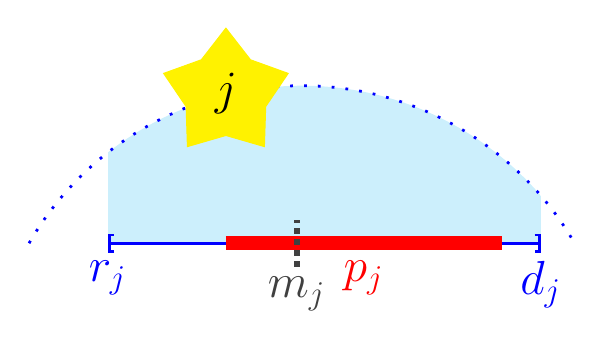
\begin{tikzpicture}
      \def\mypath{(0,0) arc[x radius=4cm, y radius=4cm, start angle=150, end angle=30]};

      \begin{scope}
        \clip\mypath;
        \fill[fill=cyan!20!] (1,0) rectangle (6.5,2.5);
      \end{scope}

      \draw[line width=1pt, color=blue, loosely dotted] \mypath;

      \node[star, star point height=3mm, minimum size=5mm, draw,
      color=yellow,fill=yellow,text=black] at (2.5,1.9) {\LARGE $j$};

      \draw[line width=1pt,color=blue,arrows={Bracket-Bracket}] (1,0)--(6.5,0);
      \node[below,blue] at (1,-.1) {\LARGE $r_j$};
      \node[below,blue] at (6.5,-.1) {\LARGE $d_j$};
      \draw[line width=5pt, color=red] (2.5,0) -- (6,0);
      \node[below,red] at (4.25,-.1) {\LARGE $p_j$};
      \draw[line width=2pt,dotted,darkgray](3.4,-0.3)--(3.4,0.3);
      \node[below,darkgray] at (3.4,-0.3) {\LARGE $m_j$};
    \end{tikzpicture}
  \end{minipage}
  \hfill
  \begin{minipage}{.26\linewidth}\footnotesize
    \begin{itemize}
      \item $\interval[open right]{r_j}{d_j}$: visibility interval
      \item $p_j$: observation time
      \item $w_j$: scientific interest of the observation
    \end{itemize}
  \end{minipage}

  \vfill

  Every observation $j$ has a meridian $m_j \in \interval[open right]{r_j}{d_j}$ which is a \alert{mandatory instant} of the observation.
\end{frame}

\begin{frame}
  \frametitle{Problem definition}

  Instance: a set of stars \alert{$\cal N$}; each star $j\in\cal N$ has a scientific interest \alert{$w_j$}, an observation time \alert{$p_j$} and a time window \alert{$\interval[open right]{r_j}{d_j}$}

  \vfill

  \alt<1>{%
    \begin{tikzpicture}
      % \mystar{y}{r}{d-r}{t-r}{p}{nom}
      \mystar{1.5}{0}{6}{1}{4}{$1$}{1}
      \mystar{1.5}{7}{3}{.5}{2}{$2$}{1}
      \mystar{1.0}{3}{6}{1}{4}{$3$}{1}
      \mystar{0.5}{1}{4}{0.9}{2.2}{$4$}{1}
      \mystar{0.5}{7}{2.5}{0.5}{1.5}{$5$}{1}
      \mystar{0}{4}{5}{1}{3}{$6$}{1}
    \end{tikzpicture}
  }{%
    \begin{tikzpicture}
      % \mystar{y}{r}{d-r}{t-r}{p}{nom}
      \mystar{1.5}{0}{6}{0}{4}{$1$}{1}
      \mystar{1.5}{7}{3}{.5}{2}{$2$}{.2}
      \mystar{1.0}{3}{6}{1}{4}{$3$}{1}
      \mystar{0.5}{1}{4}{0.9}{2.2}{$4$}{.2}
      \mystar{0.5}{7}{2.5}{1}{1.5}{$5$}{1}
      \mystar{0}{4}{5}{1}{3}{$6$}{.1}
    \end{tikzpicture}
  }

  \vfill

  \visible<2->{%
    Problem: find a subset $\cal \alert{N'} \subset N$ as well as the start date \alert{$s_j$} of each selected observation $j \in \cal{N}'$ such that:
    \begin{itemize}
      \item for all $j\in\cal N'$: $\interval[open right]{s_j}{s_j + p_j} \subset \interval[open right]{r_j}{d_j}$
      \item for all $(j_1,j_2)\in{\cal N'}^2: \interval[open right]{s_{j_1}}{s_{j_1} + p_{j_1}} \cap \interval[open right]{s_{j_2}}{s_{j_2} + p_{j_2}} = \emptyset$
    \end{itemize}
    Objective: maximize $\sum_{j\in\cal N'} w_j$ the profit of the selected observations.
  }
\end{frame}

\begin{frame}
  \frametitle{Properties}

  \begin{block}{Property 1}
    There exists an optimal solution in which selected observations are scheduled in non-decreasing order of their mandatory instant.
  \end{block}

  \pause

  \begin{center}%
    \temporal<3>{%
      \begin{tikzpicture}
        \mystar{0.5}{0}{3.5}{0.875}{1.75}{$j_1$}{1}
        \mystar{0.0}{1}{6}{1.5}{3}{$j_2$}{1}
        \draw[line width=2pt,dotted,darkgray]%
        (2.15, 0.2)--(2.15,0.8)
        (4.4,-0.3)--(4.4,0.3);
      \end{tikzpicture}
    }{%
      
\begin{tikzpicture}
        \mystar{0.5}{0}{3.5}{1.75}{1.75}{$j_1$}{1}
        \mystar{0.0}{1}{6}{0}{3}{$j_2$}{1}
        \draw[line width=2pt,dotted,darkgray]%
        (2.15, 0.2)--(2.15,0.8)
        (4.4,-0.3)--(4.4,0.3);
        \draw[line width=3pt,black] (2.15,0.5)--+(1.75,0) (2.15,0)--+(1.75,0);
        \draw[line width=2pt,red] (2.27,0.7)--(3.78,-0.2) (2.27,-0.2)--(3.78,0.7);
      \end{tikzpicture}
    }{%
      \begin{tikzpicture}
        \mystar{0.5}{0}{3.5}{0}{1.75}{$j_1$}{1}
        \mystar{0.0}{1}{6}{2.95}{3}{$j_2$}{1}
        \draw[line width=2pt,dotted,darkgray]%
        (2.15, 0.2)--(2.15,0.8)
        (4.4,-0.3)--(4.4,0.3);
      \end{tikzpicture}
    }
  \end{center}

  \onslide<5>{%
    \begin{block}{Property 2}
      Consider a subset $\cal N' \subset N$ and an observation $j_\text{max}$ such that $d_{j_\text{max}} = \max_{j \in \cal N'} d_j$.
      If there exists a feasible solution with selected observations $\cal N'$, then there exists a feasible solution with selected observations $\cal N'$ such that $s_{j_\text{max}} = d_{j_\text{max}} - p_{j_\text{max}}$.
    \end{block}
  }
  \pause
\end{frame}

\begin{frame}
  \frametitle{Recursive function}
  \small

  We consider than the observations are numbered in non-decreasing order of their mandatory instant.

  \bigskip

  \pause
  For all $j = 0, \dots, n$, $t = 0, \dots, T$, let us define \alert{$F(j, t)$} the maximum scientific interest of a subset of observations of $1, \dots, j$ during the interval $\interval[]{0}{T}$.

  \pause
  \begin{displaymath}
    F(j, t) = 
    \left\{
      \begin{array}{ll}
        0 & j = 0 \\
        F(j - 1, t) & j \neq 0, t \in \interval[open right]{0}{r_j + p_j} \\
          \max \left\{ 
            \begin{array}{l}
              F(j - 1, t)	 \\
              F(j - 1, \min\{d_j, t\} - p_j) + w_j
            \end{array}
            \right. & \text{otherwise} \\
      \end{array}
    \right.
  \end{displaymath}

  \pause
  Complexity: $O(nT)$

  \bigskip

  \pause
  Sometimes, a bit of work is needed in order to exhibit the structure to design an efficient algorithm based on dynamic programming.
\end{frame}

\section{Dynamic programming as a tree search}

\begin{frame}
  \frametitle{Breadth first search: example (knapsack problem)}

  \begin{minipage}[t]{0.48\linewidth}
    Example:

    $C = 5$
  \end{minipage}
  \begin{minipage}[t]{0.48\linewidth}
    \tiny
    \begin{center}
      \begin{tabular}{ccc}
        \toprule
        Item & Weight & Profit \\
        \midrule
        1 & 3 & 2 \\
        2 & 2 & 2 \\
        3 & 2 & 3 \\
        4 & 1 & 2 \\
        \bottomrule
      \end{tabular}
    \end{center}
  \end{minipage}

  \pause

  \begin{center}
    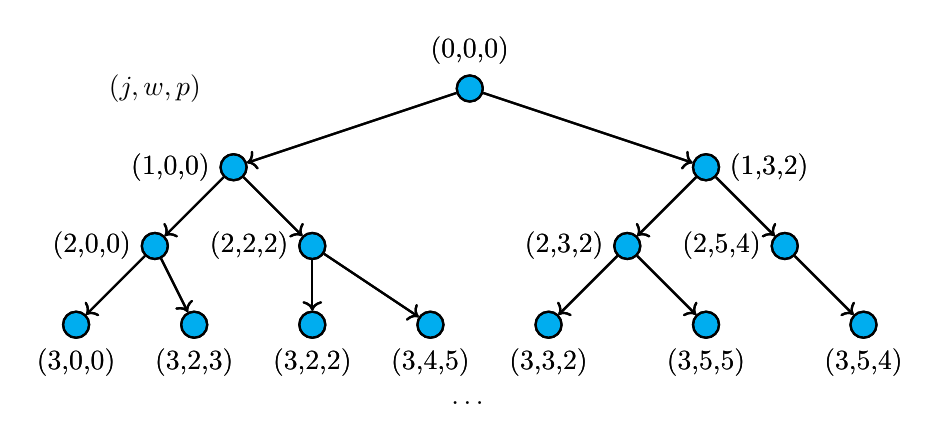
\begin{tikzpicture}
      \node[] (N0) at (-4, 0) {$(j, w, p)$};

      \onslide<2>{\node[draw=black, thick, circle, fill=cyan, label=above:{(0,0,0)}] (N1) at (0,0) {};}
        \onslide<3->{\node[draw=black, thick, circle, label=above:{(0,0,0)}] (N1) at (0,0) {};}

      \onslide<3>{%
        \node[draw=black, thick, circle, fill=cyan, label=left:{(1,0,0)}] (N11) at (-3,-1) {};
        \node[draw=black, thick, circle, fill=cyan, label=right:{(1,3,2)}] (N12) at (3,-1) {};
        \draw [thick, draw=black, ->] (N1) -- (N11);
        \draw [thick, draw=black, ->] (N1) -- (N12);
      }
      \onslide<4->{%
        \node[draw=black, thick, circle, label=left:{(1,0,0)}] (N11) at (-3,-1) {};
        \node[draw=black, thick, circle, label=right:{(1,3,2)}] (N12) at (3,-1) {};
        \draw [thick, draw=black, ->] (N1) -- (N11);
        \draw [thick, draw=black, ->] (N1) -- (N12);
      }

      \onslide<4>{%
        \node[draw=black, thick, circle, fill=cyan, label=left:{(2,0,0)}] (N111) at (-4,-2) {};
        \node[draw=black, thick, circle, fill=cyan, label=left:{(2,2,2)}] (N112) at (-2,-2) {};
        \draw [thick, draw=black, ->] (N11) -- (N111);
        \draw [thick, draw=black, ->] (N11) -- (N112);

        \node[draw=black, thick, circle, fill=cyan, label=left:{(2,3,2)}] (N121) at (2,-2) {};
        \node[draw=black, thick, circle, fill=cyan, label=left:{(2,5,4)}] (N122) at (4,-2) {};
        \draw [thick, draw=black, ->] (N12) -- (N121);
        \draw [thick, draw=black, ->] (N12) -- (N122);
      }
      \onslide<5->{%
        \node[draw=black, thick, circle, label=left:{(2,0,0)}] (N111) at (-4,-2) {};
        \node[draw=black, thick, circle, label=left:{(2,2,2)}] (N112) at (-2,-2) {};
        \draw [thick, draw=black, ->] (N11) -- (N111);
        \draw [thick, draw=black, ->] (N11) -- (N112);

        \node[draw=black, thick, circle, label=left:{(2,3,2)}] (N121) at (2,-2) {};
        \node[draw=black, thick, circle, label=left:{(2,5,4)}] (N122) at (4,-2) {};
        \draw [thick, draw=black, ->] (N12) -- (N121);
        \draw [thick, draw=black, ->] (N12) -- (N122);
      }
      \onslide<5>{%
        \node[draw=black, thick, circle, fill=cyan, label=below:{(3,0,0)}] (N1111) at (-5,-3) {};
        \node[draw=black, thick, circle, fill=cyan, label=below:{(3,2,3)}] (N1112) at (-3.5,-3) {};
        \draw [thick, draw=black, ->] (N111) -- (N1111);
        \draw [thick, draw=black, ->] (N111) -- (N1112);

        \node[draw=black, thick, circle, fill=cyan, label=below:{(3,2,2)}] (N1121) at (-2,-3) {};
        \node[draw=black, thick, circle, fill=cyan, label=below:{(3,4,5)}] (N1122) at (-0.5,-3) {};
        \draw [thick, draw=black, ->] (N112) -- (N1121);
        \draw [thick, draw=black, ->] (N112) -- (N1122);

        \node[draw=black, thick, circle, fill=cyan, label=below:{(3,3,2)}] (N1211) at (1,-3) {};
        \node[draw=black, thick, circle, fill=cyan, label=below:{(3,5,5)}] (N1212) at (3,-3) {};
        \draw [thick, draw=black, ->] (N121) -- (N1211);
        \draw [thick, draw=black, ->] (N121) -- (N1212);

        \node[draw=black, thick, circle, fill=cyan, label=below:{(3,5,4)}] (N1221) at (5,-3) {};
        \draw [thick, draw=black, ->] (N122) -- (N1221);
      }
      \onslide<6->{%
        \node[draw=black, thick, circle, label=below:{(3,0,0)}] (N1111) at (-5,-3) {};
        \node[draw=black, thick, circle, label=below:{(3,2,3)}] (N1112) at (-3.5,-3) {};
        \draw [thick, draw=black, ->] (N111) -- (N1111);
        \draw [thick, draw=black, ->] (N111) -- (N1112);

        \node[draw=black, thick, circle, label=below:{(3,2,2)}] (N1121) at (-2,-3) {};
        \node[draw=black, thick, circle, label=below:{(3,4,5)}] (N1122) at (-0.5,-3) {};
        \draw [thick, draw=black, ->] (N112) -- (N1121);
        \draw [thick, draw=black, ->] (N112) -- (N1122);

        \node[draw=black, thick, circle, label=below:{(3,3,2)}] (N1211) at (1,-3) {};
        \node[draw=black, thick, circle, label=below:{(3,5,5)}] (N1212) at (3,-3) {};
        \draw [thick, draw=black, ->] (N121) -- (N1211);
        \draw [thick, draw=black, ->] (N121) -- (N1212);

        \node[draw=black, thick, circle, label=below:{(3,5,4)}] (N1221) at (5,-3) {};
        \draw [thick, draw=black, ->] (N122) -- (N1221);
      }
      \onslide<6->{%
        \node[] (N0) at (0,-4) {\dots};
      }
    \end{tikzpicture}
  \end{center}
\end{frame}

\begin{frame}
  \frametitle{Breadth first search (knapsack problem)}

  \begin{algorithmic}
    \Procedure{BreadthFirstSearch}{w, C}
    \State$L_0 \gets ((0, 0, 0))$
    \For {$k = 1, \dots, n$}
    \For {$(j, w, p) \in L_{k - 1}$}
    \State {$L_k \gets L_k \cup ((j + 1, w, p)) $}
    \If {$w + w_{j + 1} \le C$}
    \State {$L_k \gets L_k \cup ((j + 1, w + w_{j + 1}, p + p_{j + 1})) $}
    \EndIf
    \EndFor
    \EndFor
    \EndProcedure{}
  \end{algorithmic}

  \begin{itemize}
    \item \pause Time complexity? \pause $O(2^n)$
    \item \pause Space complexity? \pause $O(2^n)$
  \end{itemize}

\end{frame}

\begin{frame}
  \frametitle{Dominance rule (knapsack problem)}

  We express dynamic programming as a dominance rule:
  Consider two nodes $n_1 = (j_1, w_1, p_1)$ and $n_2 = (j_2, w_2, p_2)$.
  If
  \begin{displaymath}
    j_1 \le j_2 \quad \text{and} \quad w_1 \le w_2 \quad \text{and} \quad p_1 \ge p_2
  \end{displaymath}
  then node $n_1$ dominates node $n_2$ and therefore node $n_2$ can be safely pruned.
\end{frame}

\begin{frame}
  \frametitle{Breadth first search + dominance rule: example (knapsack problem)}

  \begin{minipage}[t]{0.48\linewidth}
    Example:

    $C = 5$
  \end{minipage}
  \begin{minipage}[t]{0.48\linewidth}
    \tiny
    \begin{center}
      \begin{tabular}{ccc}
        \toprule
        Item & Weight & Profit \\
        \midrule
        1 & 3 & 2 \\
        2 & 2 & 2 \\
        3 & 2 & 3 \\
        4 & 1 & 2 \\
        \bottomrule
      \end{tabular}
    \end{center}
  \end{minipage}

  \pause

  \begin{center}
    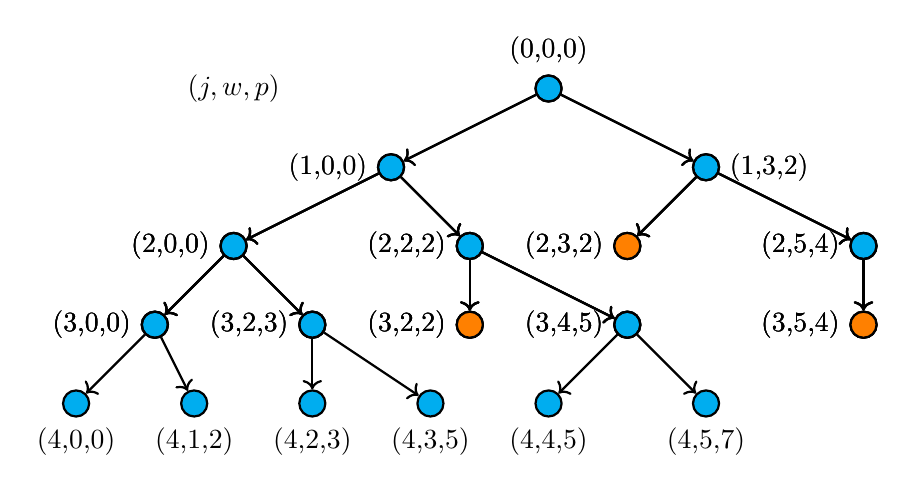
\begin{tikzpicture}
      \node[] (N0) at (-4, 0) {$(j, w, p)$};

      \onslide<2>{\node[draw=black, thick, circle, fill=cyan, label=above:{(0,0,0)}] (N1) at (0,0) {};}
        \onslide<3->{\node[draw=black, thick, circle, label=above:{(0,0,0)}] (N1) at (0,0) {};}

      \onslide<3>{%
        \node[draw=black, thick, circle, fill=cyan, label=left:{(1,0,0)}] (N11) at (-2,-1) {};
        \node[draw=black, thick, circle, fill=cyan, label=right:{(1,3,2)}] (N12) at (2,-1) {};
        \draw [thick, draw=black, ->] (N1) -- (N11);
        \draw [thick, draw=black, ->] (N1) -- (N12);
      }
      \onslide<4->{%
        \node[draw=black, thick, circle, label=left:{(1,0,0)}] (N11) at (-2,-1) {};
        \node[draw=black, thick, circle, label=right:{(1,3,2)}] (N12) at (2,-1) {};
        \draw [thick, draw=black, ->] (N1) -- (N11);
        \draw [thick, draw=black, ->] (N1) -- (N12);
      }

      \onslide<4>{%
        \node[draw=black, thick, circle, fill=cyan, label=left:{(2,0,0)}] (N111) at (-4,-2) {};
        \node[draw=black, thick, circle, fill=cyan, label=left:{(2,2,2)}] (N112) at (-1,-2) {};
        \draw [thick, draw=black, ->] (N11) -- (N111);
        \draw [thick, draw=black, ->] (N11) -- (N112);

        \node[draw=black, thick, circle, fill=cyan, label=left:{(2,3,2)}] (N121) at (1,-2) {};
        \node[draw=black, thick, circle, fill=cyan, label=left:{(2,5,4)}] (N122) at (4,-2) {};
        \draw [thick, draw=black, ->] (N12) -- (N121);
        \draw [thick, draw=black, ->] (N12) -- (N122);
      }
      \onslide<5>{%
        \node[draw=black, thick, circle, fill=cyan, label=left:{(2,0,0)}] (N111) at (-4,-2) {};
        \node[draw=black, thick, circle, fill=cyan, label=left:{(2,2,2)}] (N112) at (-1,-2) {};
        \draw [thick, draw=black, ->] (N11) -- (N111);
        \draw [thick, draw=black, ->] (N11) -- (N112);

        \node[draw=black, thick, circle, fill=orange, label=left:{(2,3,2)}] (N121) at (1,-2) {};
        \node[draw=black, thick, circle, fill=cyan, label=left:{(2,5,4)}] (N122) at (4,-2) {};
        \draw [thick, draw=black, ->] (N12) -- (N121);
        \draw [thick, draw=black, ->] (N12) -- (N122);
      }
      \onslide<6->{%
        \node[draw=black, thick, circle, label=left:{(2,0,0)}] (N111) at (-4,-2) {};
        \node[draw=black, thick, circle, label=left:{(2,2,2)}] (N112) at (-1,-2) {};
        \draw [thick, draw=black, ->] (N11) -- (N111);
        \draw [thick, draw=black, ->] (N11) -- (N112);

        \node[draw=black, thick, circle, fill=orange, label=left:{(2,3,2)}] (N121) at (1,-2) {};
        \node[draw=black, thick, circle, label=left:{(2,5,4)}] (N122) at (4,-2) {};
        \draw [thick, draw=black, ->] (N12) -- (N121);
        \draw [thick, draw=black, ->] (N12) -- (N122);
      }
      \onslide<6>{%
        \node[draw=black, thick, circle, fill=cyan, label=left:{(3,0,0)}] (N1111) at (-5,-3) {};
        \node[draw=black, thick, circle, fill=cyan, label=left:{(3,2,3)}] (N1112) at (-3,-3) {};
        \draw [thick, draw=black, ->] (N111) -- (N1111);
        \draw [thick, draw=black, ->] (N111) -- (N1112);

        \node[draw=black, thick, circle, fill=cyan, label=left:{(3,2,2)}] (N1121) at (-1,-3) {};
        \node[draw=black, thick, circle, fill=cyan, label=left:{(3,4,5)}] (N1122) at (1,-3) {};
        \draw [thick, draw=black, ->] (N112) -- (N1121);
        \draw [thick, draw=black, ->] (N112) -- (N1122);

        \node[draw=black, thick, circle, fill=cyan, label=left:{(3,5,4)}] (N1221) at (4,-3) {};
        \draw [thick, draw=black, ->] (N122) -- (N1221);
      }
      \onslide<7>{%
        \node[draw=black, thick, circle, fill=cyan, label=left:{(3,0,0)}] (N1111) at (-5,-3) {};
        \node[draw=black, thick, circle, fill=cyan, label=left:{(3,2,3)}] (N1112) at (-3,-3) {};
        \draw [thick, draw=black, ->] (N111) -- (N1111);
        \draw [thick, draw=black, ->] (N111) -- (N1112);

        \node[draw=black, thick, circle, fill=orange, label=left:{(3,2,2)}] (N1121) at (-1,-3) {};
        \node[draw=black, thick, circle, fill=cyan, label=left:{(3,4,5)}] (N1122) at (1,-3) {};
        \draw [thick, draw=black, ->] (N112) -- (N1121);
        \draw [thick, draw=black, ->] (N112) -- (N1122);

        \node[draw=black, thick, circle, fill=orange, label=left:{(3,5,4)}] (N1221) at (4,-3) {};
        \draw [thick, draw=black, ->] (N122) -- (N1221);
      }
      \onslide<8->{%
        \node[draw=black, thick, circle, label=left:{(3,0,0)}] (N1111) at (-5,-3) {};
        \node[draw=black, thick, circle, label=left:{(3,2,3)}] (N1112) at (-3,-3) {};
        \draw [thick, draw=black, ->] (N111) -- (N1111);
        \draw [thick, draw=black, ->] (N111) -- (N1112);

        \node[draw=black, thick, circle, fill=orange, label=left:{(3,2,2)}] (N1121) at (-1,-3) {};
        \node[draw=black, thick, circle, label=left:{(3,4,5)}] (N1122) at (1,-3) {};
        \draw [thick, draw=black, ->] (N112) -- (N1121);
        \draw [thick, draw=black, ->] (N112) -- (N1122);

        \node[draw=black, thick, circle, fill=orange, label=left:{(3,5,4)}] (N1221) at (4,-3) {};
        \draw [thick, draw=black, ->] (N122) -- (N1221);
      }
      \onslide<8>{%
        \node[draw=black, thick, circle, fill=cyan, label=below:{(4,0,0)}] (N11111) at (-6,-4) {};
        \node[draw=black, thick, circle, fill=cyan, label=below:{(4,1,2)}] (N11112) at (-4.5,-4) {};
        \draw [thick, draw=black, ->] (N1111) -- (N11111);
        \draw [thick, draw=black, ->] (N1111) -- (N11112);

        \node[draw=black, thick, circle, fill=cyan, label=below:{(4,2,3)}] (N11121) at (-3,-4) {};
        \node[draw=black, thick, circle, fill=cyan, label=below:{(4,3,5)}] (N11122) at (-1.5,-4) {};
        \draw [thick, draw=black, ->] (N1112) -- (N11121);
        \draw [thick, draw=black, ->] (N1112) -- (N11122);

        \node[draw=black, thick, circle, fill=cyan, label=below:{(4,4,5)}] (N11221) at (0,-4) {};
        \node[draw=black, thick, circle, fill=cyan, label=below:{(4,5,7)}] (N11222) at (2,-4) {};
        \draw [thick, draw=black, ->] (N1122) -- (N11221);
        \draw [thick, draw=black, ->] (N1122) -- (N11222);
      }
    \end{tikzpicture}
  \end{center}
\end{frame}

\begin{frame}
  \frametitle{Breadth first search + dominance rule (knapsack problem)}

  \begin{algorithmic}
    \Procedure{BreadthFirstSearch}{w, C}
    \State $L_0 \gets ((0, 0, 0))$
    \For {$k = 1, \dots, n$}
    \For {$(j, w, p) \in L_{k - 1}$}
    \State $L_k \gets L_k \cup ((j + 1, w, p)) $
    \If {$w + w_{j + 1} \le C$}
    \State $L_k \gets L_k \cup ((j + 1, w + w_{j + 1}, p + p_{j + 1}))$
    \EndIf
    \EndFor
    \State \alert{Remove all dominated nodes from $L_j$}
    \EndFor
    \EndProcedure
  \end{algorithmic}

  \begin{itemize}
    \item \pause Time complexity? \pause The complexity depends on the complexity of applying the dominance rule!

  In this case, it is possible to implement it in $O(C)$ and keep the complexity of the whole algorithm to $O(nC)$ as for the iterative implementation. But in some cases, the complexity might increase.
  \end{itemize}
\end{frame}

\section{Conclusion}

\begin{frame}
  \frametitle{Conclusion}

  \begin{itemize}
    \item Dynamic programming: solving a problem recursively and storing the results of the subproblems to avoid recomputing them multiple times.
    \item It requires the problem to have a specific structure. It might not be applicable to all problems.
    \item Sometimes, a bit of work is needed in order to exhibit this structure
    \item Multiple possible implementations with their advantages and drawbacks (recursive, iterative, tree search)
    \item \say{Knapsack Problems} (Kellerer, Pferschy et Pisinger, 2004)
    \item Dynamic programming through path problems: \url{https://moodle.caseine.org/mod/page/view.php?id=30723}
  \end{itemize}

\end{frame}

\maketitle

\end{document}

